\documentclass[pra,amsfonts,showpacs,preprint,showkeys]{revtex4}
%\documentclass[pra,showpacs,showkeys,amsfonts]{revtex4}
\usepackage{graphicx}
\usepackage{amsmath}
%\documentstyle[amsfonts]{article}
\RequirePackage{times}
%\RequirePackage{courier}
\RequirePackage{mathptm}
%\renewcommand{\baselinestretch}{1.3}

\begin{document}
%\sloppy



\title{Nonlocal four-partite quantum correlations of singlet states}

\author{Boris Kamenik}
\author{Karl Svozil}
\email{svozil@tuwien.ac.at}
\homepage{http://tph.tuwien.ac.at/~svozil}
\affiliation{Institut f\"ur Theoretische Physik, University of Technology Vienna,
Wiedner Hauptstra\ss e 8-10/136, A-1040 Vienna, Austria}

\begin{abstract}
The correlations of four spin-$\frac{1}{2}$ particles in the two singlet states are investigated for their use in quantum communication. Multipartite quantized systems can be partitioned, and their observables grouped and redefined into condensed correlations.
\end{abstract}

\pacs{03.67.Hk,03.65.Ud,03.65.Ta,03.67.Mn}
\keywords{Quantum information, entanglement, quantum nonlocality}

\maketitle


%\section{Introduction}

One of the advantages of quantum computation and communication \cite{nielsen-book,Gruska,benn:97,Ozhigov:1997,bbcmw-01,cleve-99,fortnov-03}
over classical algorithms and protocols \cite{rogers1,odi:89} is based upon
the fact that in quantum mechanics information
can be coded in or ``spread among'' coherent nonlocal multipartite states in such a way that
its retreival must be nonlocal as well.
In that way, information is ``stored collectively'' among the participating quanta.
It can be retreived only by joint measurements \cite{DonSvo01,svozil-2002-statepart-prl}.

This nonlocal form of encoding information motivates the study of multipartite correlations,
which is also stimulated by improved experimental particle production methods.
In what follows, we present an explicit analysis of the singlet states of
four spin-$\frac{1}{2}$ particles in terms of their probabilities and
expectation functions for spin state measurements.
We also investigate the possibility to group the outcomes
of the four spin state measurements on each particle to obtain ``condensed''
observables.
One of our physical motivations for doing so was the question of how such ``condensed'' observables
would perform with respect to violations of classical locality conditions.

%\section{States}
To begin with the analysis, consider four spin-${1\over 2}$
particles in one of the two singlet states
\begin{eqnarray}
\vert \Psi_{4,s_1} \rangle
&=&
\left( \vert \Psi_{2,s} \rangle \right)^2
=
{1\over 2}
\bigl(
\vert +- \rangle -
\vert -+ \rangle
\bigr)
\bigl(
\vert +- \rangle -
\vert -+ \rangle
\bigr),
\label{2004-gtq-s1}
\\
\vert \Psi_{4,s_2} \rangle
&=&
{1\over \sqrt{3}}\Bigl[
\vert ++-- \rangle +
\vert --++ \rangle \nonumber \\
&&\qquad
\qquad
-  {1\over 2}
\bigl(
\vert +- \rangle +
\vert -+ \rangle
\bigr)
\bigl(
\vert +- \rangle +
\vert -+ \rangle
\bigr)
\Bigr].
\label{2005-hp-ep24s2}
\end{eqnarray}
where
$\vert \Psi_{2,s} \rangle = \frac{1}{\sqrt{ 2}}
\bigl(
\vert +- \rangle -
\vert -+ \rangle
\bigr)
$
is the two particle singlet state.
With
$
\vert +\rangle
$
corresponding to
$ {\hat {\bf e}}_1 =(1,0)
$
and
$
\vert -\rangle $
corresponding to
${\hat {\bf e}}_2 =(0,1)
$,
the two pure states have a vector representation as
\begin{eqnarray}
\hat  \Psi_{4,s_1}
 &=&
{1\over \sqrt{2}}\bigl({\hat {\bf e}}_1\otimes {\hat {\bf e}}_2-{\hat {\bf e}}_2\otimes {\hat {\bf e}}_1 \bigr)
\otimes
 {1\over \sqrt{2}}\bigl({\hat {\bf e}}_1\otimes {\hat {\bf e}}_2-{\hat {\bf e}}_2\otimes {\hat {\bf e}}_1 \bigr)
\nonumber \\
&=&\left( 0,0,0,0,0,\frac{1}{2},- \frac{1}{2} ,  0,0,- \frac{1}{2} ,\frac{1}{2},0,0,0,0,  0\right),
\label{2005-hp-ep24s1v}
\\
\hat  \Psi_{4,s_2}
&=&
{1\over \sqrt{3}}\Bigl[
{\hat {\bf e}}_1\otimes {\hat {\bf e}}_1\otimes {\hat {\bf e}}_2\otimes {\hat {\bf e}}_2+
{\hat {\bf e}}_2\otimes {\hat {\bf e}}_2\otimes {\hat {\bf e}}_1\otimes {\hat {\bf e}}_1
 \nonumber \\
&&\qquad
-  {1\over \sqrt{2}}\bigl({\hat {\bf e}}_1\otimes {\hat {\bf e}}_2+{\hat {\bf e}}_2\otimes {\hat {\bf e}}_1 \bigr)
\otimes
 {1\over \sqrt{2}}\bigl({\hat {\bf e}}_1\otimes {\hat {\bf e}}_2+{\hat {\bf e}}_2\otimes {\hat {\bf e}}_1 \bigr)
\Bigr]\nonumber \\
&=&\left( 0,0,0,\frac{1}{{\sqrt{3}}},0,
  -\frac{1}{2\,{\sqrt{3}}},-\frac{1}{2\,{\sqrt{3}}},0,
  0,-\frac{1}{2\,{\sqrt{3}}},-\frac{1}{2\,{\sqrt{3}}},
  0,\frac{1}{{\sqrt{3}}},0,0,0\right).
\label{2005-hp-ep24s2v}
\end{eqnarray}
Their density operators $\rho_{i}$, $i=1,2$
are just the projectors corresponding to the one-dimensional
linear subspaces spanned by
the vectors representing
$ \hat \Psi_{4,s_1}$
and
$\hat \Psi_{4,s_2}$
in Eqs.~(\ref{2005-hp-ep24s1v},~\ref{2005-hp-ep24s2v}); i.\,e.
they are  the dyadic product
\begin{equation}
%\begin{array}{lll}
\rho_{i} = \left[ {\hat \Psi}_{4,s_i}^T {\hat \Psi}_{4,s_i}\right].
%\end{array}
\end{equation}

As $ \hat \Psi_{4,s_1}\cdot \hat \Psi_{4,s_2}=0$
or equivalently $\rho_{1}\cdot \rho_{2} = 0$,
the singlet states are orthogonal.
The most general form of a four spin-${1\over 2}$
particle singlet state is
thus given by
\begin{equation}
\vert \Psi_{4,s} \rangle
= \lambda_1 \;
\vert \Psi_{4,s_1} \rangle
+
\lambda_2   \;
\vert \Psi_{4,s_2} \rangle
\label{2005-hp-ep24smgf}
\end{equation}
with
$
\vert \lambda_1 \vert^2
+
\vert \lambda_2 \vert^2
=1
$,
which can be parameterized by
$\lambda_1=\cos \tau $,
$\lambda_2=\sin \tau $.

It is easily shown that for integer multiples of $\tau = \frac{\pi}{3}$,
like in $\vert \Psi_{4,s_1} \rangle$, the singlet state takes the
form of a product of two two-partite singlet states involving varying
particles (Eqs.~(\ref{2005-gtq-psi1equi1}--\ref{2005-gtq-psi1equi3})).
Entanglement will only be among the particles within those factors,
not across factors.
\begin{eqnarray}
\label{2005-gtq-psi1equi1}
\vert \Psi_{4,s} (\tau = \frac{\pi}{3}) \rangle &=& \mathcal{P}_{2,3} \vert \Psi_{4,s} (\tau=0) \rangle\\
\label{2005-gtq-psi1equi2}
\vert \Psi_{4,s} (\tau = 2 \frac{\pi}{3}) \rangle &=& \mathcal{P}_{2,4} \vert \Psi_{4,s} (\tau= \frac{\pi}{3}) \rangle\\
\label{2005-gtq-psi1equi3}
\vert \Psi_{4,s} (\tau = \pi) \rangle &=& - \vert \Psi_{4,s} (\tau = 0) \rangle
\end{eqnarray}
$\mathcal{P}_{i,j}$ here is the exchange operator for particles i and j.
More complex behaviors can be expected from states like $\vert \Psi_{4,s_2} \rangle$,
involving an entanglement of all four particles \cite{krenn1}.

Singlet states are form invariant with respect to arbitrary unitary
transformations in the single-particle Hilbert spaces and thus
also rotationally invariant in configuration space,
in particular under the rotations
$
\vert \pm \rangle =
e^{\pm i{\frac{\varphi}{2}} }
\left[
\cos (\frac{\theta}{2}) \vert \chi_+ (\theta , \varphi)  \rangle
\mp
\cos (\frac{\theta}{2}) \vert \chi_- (\theta , \varphi)  \rangle
\right]
$
in the spherical coordinates $\theta , \varphi$ defined below
[e.\,g., Ref.~\cite{krenn1}, Eq.~(2), or Ref.~\cite{ba-89}, Eq.~(7--49)].
However, despite this form invariance under rotations,
the states are non-unique in the sense that knowledge
of a spin state observable for one particle is not sufficient
for the simultaneous (counterfactual) determination of
spin state properties for all other three particles
\cite{epr, svozil-2004-vax}.

%However, despite this desirable form invariance under rotations,
%the states are nonunique in the sense that knowledge
%of a spin state observable of one particle
%is not sufficient
%for the simultaneous (counterfactual) existence of elements of physical reality
%\cite{epr} on (any one) of the other three particles
%\cite{svozil-2004-vax}.
%(unklar formuliert, stimmt ausserdem nicht f�r tau = n pi/3)


%\section{Operators}

In what follows, the operators corresponding to the spin state observables will be enumerated.
Thereby, spherical coordinates represent angles of spin state measurements.
Suppose  that $i$ denotes the $i$'th particle
%and the $i$'th measurement
with $1\le i\le 4$.
Let $\theta_i$ be the polar angle in the $x$--$z$-plane
from the $z$-axis with $0 \le \theta_i \le \pi$,
and $\varphi_i$  the azimuthal angle in the $x$-$y$-plane
from the $x$-axis with $0 \le \varphi_i < 2 \pi$.
%(We will stick to the unit sphere with the distance (radius) $r=1$
%of any point on the surface to the origin of the sphere.)

%Suppose that all of the four particles propagate along the (negative) $y$-axis.
For the sake of simplicity, we shall sometimes consider measurements
in the $x$-$z$-plane, for which $\varphi_1=\varphi_2=\varphi_3=\varphi_4=0$.
Because of the spherical symmetry of the singlet state, this is in every aspect
equivalent to a measurement along angles lying in an arbitrary plane.
In such cases the expectation values (the raw, or uncentered,
product moments \cite{gill-03}) are merely functions of the polar angles
$\theta_1 $,
$\theta_2 $,
$\theta_3 $ and
$\theta_4 $,
so the azimuthal angles will be omitted.
For compact notation,
${\hat \theta}$~and~${\hat \varphi}$ will be used to denote the coordinates
$\theta_1 ,\theta_2 ,\theta_3 ,\theta_4$ and
$\varphi_1 ,\varphi_2 ,\varphi_3 ,\varphi_4$,
respectively.


The projection operators $F$
corresponding to a four~spin-${1\over 2}$~particle joint measurement
aligned (``$+$'') or antialigned  (``$-$'') along those angles are
\begin{equation}
\begin{array}{lll}
 F_{\pm \pm \pm \pm} ({\hat \theta},{\hat \varphi} ) =
{\frac{1}{2}}\left[{\mathbb I}_2 \pm {\bf \sigma}( \theta_1,\varphi_1 )\right]
\otimes
{\frac{1}{2}}\left[{\mathbb I}_2 \pm {\bf \sigma}( \theta_2,\varphi_2 )\right] \otimes
\nonumber\\
\qquad\qquad\qquad\qquad\qquad
\otimes
{\frac{1}{2}}\left[{\mathbb I}_2 \pm {\bf \sigma}( \theta_3,\varphi_3 )\right]
\otimes
{\frac{1}{2}}\left[{\mathbb I}_2 \pm {\bf \sigma}( \theta_4,\varphi_4 )\right],
\end{array}
\label{2004-gtq-e2}
\end{equation}
with
$
{\bf \sigma}( \theta ,\varphi )=
\left(
\begin{array}{cc} \cos \theta  &e^{-i\varphi} \sin \theta   \\
  e^{i\varphi}\sin \theta  & -\cos \theta
  \end{array}
\right)
$.
For example, $F_{- + - + } ({\hat \theta},{\hat \varphi} )$ stands for the proposition
\begin{quote}
{\em `The spin state of the first particle measured along $\theta_1,\varphi_1$ is ``$-$'',
      the spin state of the second particle measured along $\theta_2,\varphi_2$ is ``$+$'',
      the spin state of the third particle measured along $\theta_3,\varphi_3$ is ``$-$'',
      and the spin state of the fourth particle measured along $\theta_4,\varphi_4$ is ``$+$''~.'
}
\end{quote}
Fig.~\ref{2005-gtq-f1} depicts a measurement configuration
for a simultaneous measurement of spins along
$\theta_1,\varphi_1 $,
$\theta_2,\varphi_2 $,
$\theta_3,\varphi_3 $ and
$\theta_4,\varphi_4 $
of the state $\Psi_{4,s_1}$.
\begin{figure}[htbp]
\begin{center}

%TexCad Options
%\grade{\off}
%\emlines{\off}
%\beziermacro{\on}
%\reduce{\on}
%\snapping{\off}
%\quality{2.00}
%\graddiff{0.01}
%\snapasp{1}
%\zoom{1.00}
\unitlength 1.0mm
\linethickness{0.4pt}
\begin{picture}(120.00,68.00)
\put(60.00,45.00){\makebox(0,0)[cc]{$\Psi_{4,s_1}$}}
\put(30.00,35.00){\makebox(0,0)[cc]{$\Psi_{2,s}$}}
\put(90.00,35.00){\makebox(0,0)[cc]{$\Psi_{2,s}$}}
\put(60.00,35.00){\circle{10.00}}
\put(56.00,32.00){\line(4,3){8.00}}
\put(64.00,32.00){\line(-4,3){8.00}}
\put(57.00,31.00){\line(-2,-1){32.00}}
\put(5.00,5.00){\oval(10.00,10.00)[l]}
\put(5.00,10.00){\line(0,-1){10.00}}
\put(2.50,5.00){\makebox(0,0)[cc]{$-$}}
\put(57.00,39.00){\line(-2,1){32.00}}
\put(5.00,48.00){\oval(10.00,10.00)[l]}
\put(5.00,43.00){\line(0,1){10.00}}
\put(2.50,48.00){\makebox(0,0)[cc]{$-$}}
\put(63.00,31.00){\line(2,-1){32.00}}
\put(63.00,39.00){\line(2,1){32.00}}
\put(5.00,20.00){\oval(10.00,10.00)[l]}
\put(5.00,25.00){\line(0,-1){10.00}}
\put(2.50,20.00){\makebox(0,0)[cc]{$+$}}
\put(5.00,63.00){\oval(10.00,10.00)[l]}
\put(5.00,58.00){\line(0,1){10.00}}
\put(2.50,63.00){\makebox(0,0)[cc]{$+$}}
\put(10.00,5.00){\framebox(10.00,15.00)[cc]{$\theta_2,\varphi_2$}}
\put(10.00,48.00){\framebox(10.00,15.00)[cc]{$\theta_1,\varphi_1$}}
\put(115.00,5.00){\oval(10.00,10.00)[r]}
\put(115.00,10.00){\line(0,-1){10.00}}
\put(117.50,5.00){\makebox(0,0)[cc]{$-$}}
\put(115.00,48.00){\oval(10.00,10.00)[r]}
\put(115.00,43.00){\line(0,1){10.00}}
\put(117.50,48.00){\makebox(0,0)[cc]{$-$}}
\put(115.00,20.00){\oval(10.00,10.00)[r]}
\put(115.00,25.00){\line(0,-1){10.00}}
\put(117.50,20.00){\makebox(0,0)[cc]{$+$}}
\put(115.00,63.00){\oval(10.00,10.00)[r]}
\put(115.00,58.00){\line(0,1){10.00}}
\put(117.50,63.00){\makebox(0,0)[cc]{$+$}}
\put(100.00,5.00){\framebox(10.00,15.00)[cc]{$\theta_4,\varphi_4$}}
\put(100.00,48.00){\framebox(10.00,15.00)[cc]{$\theta_3,\varphi_3$}}
\end{picture}
\end{center}
\caption{Simultaneous spin measurement of
the four-partite singlet state represented in Eq.~(\ref{2004-gtq-s1}).
Boxes indicate spin state analyzers such as Stern-Gerlach apparatus
oriented along the directions $\theta_1,\varphi_1 $,
$\theta_2,\varphi_2 $,
$\theta_3,\varphi_3 $ and
$\theta_4,\varphi_4 $;
their two output ports are occupied with detectors  associated
with the outcomes
``$+$''
and
``$-$'',
respectively.
\label{2005-gtq-f1}}
\end{figure}

%\section{Probabilities and expectations}

We now turn to the calculation of quantum predictions.
The joint probability to register the spins of the four particles
in state $\rho_i$
aligned or antialigned along the directions defined \mbox{by $\theta_1,\varphi_1 $,
$\theta_2,\varphi_2 $,
$\theta_3,\varphi_3 $ and
$\theta_4,\varphi_4 $} can be evaluated by a straightforward calculation
of
\begin{equation}
P_{\rho_{ i }\,\pm \pm \pm \pm} ({\hat \theta},{\hat \varphi} )=
{\rm Tr}\left[\rho_i \cdot F_{\pm \pm \pm \pm} \left({\hat \theta},{\hat \varphi} \right)\right].
\end{equation}

The expectation functions and joint probabilities to find the four particles
in an even or in an odd number of
spin-``$-$''-states when measured along $\theta_1 $, $\theta_2 $,
$\theta_3 $ and
$\theta_4 $ are
enumerated in Table~\ref{2005-gtq-2part}.
%
%\begin{equation}
%\begin{array}{lll}
%P_{\rm even}^{ 1 }({\hat \theta} )  &=&
%\frac{1}{2} \left[1+\cos (\theta_1 -\theta_2 ) \cos (\theta_3 -\theta_4 )\right],\\
%%
%P_{\rm odd}^{ 1 }({\hat \theta} )  &=&
%1 - P_{\rm even}^{ 1 }  =
%\frac{1}{2} \left[1- \cos (\theta_1 -\theta_2 ) \cos (\theta_3 -\theta_4 )\right],\\
%%
%%
%P_{\rm even}^{ 2 }({\hat \theta} )  &=&
%\frac{1}{6} \left[3+2 \cos (\theta_1 +\theta_2 -\theta_3 -\theta_4 )+\cos
%   (\theta_1 -\theta_2 ) \cos (\theta_3 -\theta_4 )\right],\\
%%
%P_{\rm odd}^{ 2 }({\hat \theta} )  &=&
%1 - P_{\rm even}^{ 2 }  =
%\frac{1}{6} \left[3-2 \cos (\theta_1 +\theta_2 -\theta_3 -\theta_4 )-\cos
%   (\theta_1 -\theta_2 ) \cos (\theta_3 -\theta_4 )\right].
%\end{array}
%  \label{2005-gtq-Probs}
%\end{equation}
%Hence, the correlation functions are given by
%\begin{eqnarray}
%E^{ 1 }({\hat \theta} )  &=& P_{\rm even}^{ 1 } - P_{\rm odd}^{ 1 }  =
%\cos (\theta_1 -\theta_2 ) \cos (\theta_3 -\theta_4 ),
%  \label{2005-gtq-Exp1}
%\\
%%
%%
%E^{ 2 }({\hat \theta} )  &=& P_{\rm even}^{ 2 } - P_{\rm odd}^{ 2 }  =
%\frac{1}{3} \left[2 \cos (\theta_1 +\theta_2 -\theta_3 -\theta_4 )+\cos
%   (\theta_1 -\theta_2 ) \cos (\theta_3 -\theta_4 )\right].
%  \label{2005-gtq-Exp2}
%\end{eqnarray}
%
For example, the expectation function of the general singlet state
in Eq.~(\ref{2005-hp-ep24smgf})
restricted to
$\varphi_1=\varphi_2=\varphi_3=\varphi_4=0$
is
\begin{equation}
\begin{array}{lll}
E(\tau  ;{\hat \theta} )  &=&
\frac{1}{3}\Bigl(
\left[ 2 + \cos (2\,\tau  ) \right] \,\cos (\theta_1  - \theta_2 )\,\cos (\theta_3  - \theta_4 )\\
&&{}+ 2\,\sin \tau
         \left[\sin \tau  \,\cos (\theta_1  + \theta_2  - \theta_3  - \theta_4 ) +
       {\sqrt{3}}\,\cos \tau  \,\sin (\theta_1  - \theta_2 )\,\sin (\theta_3  - \theta_4 ) \right]
\Bigr)
\end{array}
  \label{2005-gtq-Expmgf}
\end{equation}
For $\tau  = 0$ and $\tau = \frac{\pi}{2}$ Eq.~(\ref{2005-gtq-Expmgf})
reduces to
$E_{\rho_{ 1 }}$
and
$E_{\rho_{ 2 }}$
in Table~\ref{2005-gtq-2part}.


The plasticity of the expectation function
$E(\tau  ;{\hat \theta} )$ (which is comparable to the two-particle
expectation function $E(\theta)=-\cos \theta$\,)
for measurements in one plane can either be demonstrated by plotting
the probabilities and expectation values for selectively chosen parameters,
as depicted in Fig.~\ref{2005-gtq-fpe},
or by plotting the surface $E(\tau  ;{\hat \theta} ) = 0$
over relative measuring angles, as shown in
Fig.~\ref{2005-gtq-plots1}. In the latter case, because of the spherical
symmetry of the singlet state, one of four angles can be assumed
arbitrarily, so that every set of angles for joint measurements in
one plane corresponds to a point in the periodic interval $(-\pi, \pi)^3$.

For general $\tau$ the surface $E(\tau  ;{\hat \theta} ) = 0$ divides
the interval in two connected sets of points, corresponding to sets of
angles, where the probability of measuring an even number of
spin-``$-$''-states is greater and lesser $\frac{1}{2}$, respectively.
For $\tau = n \frac{\pi}{3}$, $n \in \mathbb{Z}$,
there are 4 such domains, separated by planes with
$E({\hat \theta}) = 0$ (Fig.~\ref{2005-gtq-plots1}).

\begin{figure}[htbp]
  \centering
\begin{tabular}{cc}
  \includegraphics[width=60mm]{2005-gtq-fr1-1.eps}&
  \includegraphics[width=60mm]{2005-gtq-fr1-2.eps}\\
\quad \qquad (a) &\quad  \quad (b)\\
  \includegraphics[width=60mm]{2005-gtq-fr1-3.eps}&
  \includegraphics[width=60mm]{2005-gtq-fr1-4.eps}\\
\quad  \qquad (c)& \quad  \qquad (d)\\
  \includegraphics[width=60mm]{2005-gtq-fr1-5.eps}&
  \includegraphics[width=60mm]{2005-gtq-fr1-6.eps}\\
\quad  \qquad (e)& \quad  \qquad (f)\\
\end{tabular}
  \caption{Probabilities and expectation values for
(a)
$\tau =0$,
$\theta_1 =\theta$,
$\theta_2 =\theta_3 =\theta_4 =0$,
(b)
$\tau =0$,
$\theta_1 =\theta$,
$\theta_2 =\theta_3  =0$,
$\theta_4 =\pi$,
(c)
$\tau =\frac{\pi}{2}$,
$\theta_1 =\theta_2 =-\theta_3 =\theta_4  =\theta$,
(d)
$\tau =\frac{\pi}{2}$,
$\theta_1 =-\theta_3 =\theta_4  =\theta$,
$\theta_2 =\frac{\pi}{4}$,
(e)
$\tau =\frac{\pi}{4}$,
$\theta_1 =-\theta_3 =\theta_4  =\theta$,
$\theta_2 =\frac{\pi}{4}$,
(f)
$\tau =\frac{\pi}{4}$,
$\theta_1 =- \theta_3=\theta_4 =\theta$,
$ \theta_2 =0$.
Dashed (dash dotted) lines indicate probabilities to find an even (odd)
number of ``$-$'' outcomes, solid lines depict expectation functions.
}
\label{2005-gtq-fpe}
\end{figure}


\begin{figure}
\centering

\begin{tabular}{cc}
\includegraphics[width=65mm]{2005-gtq-p1.eps}&
\includegraphics[width=65mm]{2005-gtq-p2.eps}\\

\includegraphics[width=65mm]{2005-gtq-p3.eps}&
\includegraphics[width=65mm]{2005-gtq-p4.eps}\\

\includegraphics[width=65mm]{2005-gtq-p5.eps}&
\includegraphics[width=65mm]{2005-gtq-p6.eps}\\
\end{tabular}

\caption{Sets of angles $\hat \theta$ [rad] for joint measurements in one plane
where $E(\tau  ;{\hat \theta} ) = 0$ for $\tau = 0$ ($\vert \Psi_{4,s_1} \rangle$),
$\tau = \frac{\pi}{100}$,
$\tau = \frac{\pi}{6}$,
$\tau = \frac{\pi}{3} - \frac{\pi}{100}$,
$\tau = \frac{\pi}{3}$ and
$\tau = \frac{\pi}{2}$ ($\vert \Psi_{4,s_2} \rangle$).
}
\label{2005-gtq-plots1}
\end{figure}


As there are four particles involved, the outcomes of one or two particles can be utilized
to select the events of the other particles. Table~\ref{2005-gtq-2partwith}
contains the results of the associated expectation values and joint probabilities
for finding an odd or even number of spin-``$-$''-states.

Two or three observables could also be grouped together to form a ``condensed'' observable.
For instance, for each individual quadruple of outcomes $\{o_1,o_2,o_3,o_4\}$
the values of the first and %the
second, as well as of the third and %the
fourth particle could be multiplied to obtain two other, dichotomic observables
$o_1o_2$ and $o_3o_4$%, respectively
. More generally, one could take all partitions of 4,
such that the outcomes of all particles within an element of the partition
are multiplied. As the single outcomes occur at random, their resulting products
and thus the new \emph{condensed observable} would also
be random. Since the multiplication is associative,
the resulting \emph{condensed correlations} are just the four-partite correlations discussed
so far.

Another interesting observable is the sum of outcomes of a joint spin state measurement,
``$+$'' and ``$-$'' counted as $+1$ and $-1$, respectively.
Its possible values are $-4$, $-2$, $0$, $2$ and $4$, so there is no obvious way
to construct something like the expectation functions for dichotomic observables.
As this \emph{sum of outcomes} is the most general observable invariant to
permutations of the particles, the joint probabilities for every other such observable
(e.\,g. the probabilities of finding an odd or even number of spin-``$-$''-states
discussed above) can be written as a sum of joint probabilities for sums of outcomes
(enumerated in Tables~\ref{2005-gtq-tabsums1}~and~\ref{2005-gtq-tabsums2} for
$\vert \Psi_{4,s_1} \rangle$ and $\vert \Psi_{4,s_2} \rangle$).

For joint measurements in one plane, the variation of the probabilities for
different sums of outcomes can be illustrated by plotting sets of relative measurement
angles, where the probability of measuring a certain sum of outcomes is equal to the
probability expected for nonentangled particles, as shown in Fig.~\ref{2005-gtq-plots2}.
These ``classical'' probabilities ($\frac{3}{8}$, $\frac{1}{4}$ and $\frac{1}{16}$)
correspond to those expected e.\,g. for the results of tossing 4 coins and counting
the number of heads or tails.


\begin{figure}
\centering

\begin{tabular}{ccc}
\includegraphics[width=52mm]{2005-gtq-ps1-0.eps}&
\includegraphics[width=52mm]{2005-gtq-ps1-2.eps}&
\includegraphics[width=52mm]{2005-gtq-ps1-4.eps}\\
\includegraphics[width=52mm]{2005-gtq-ps2-0.eps}&
\includegraphics[width=52mm]{2005-gtq-ps2-2.eps}&
\includegraphics[width=52mm]{2005-gtq-ps2-4.eps}\\
\includegraphics[width=52mm]{2005-gtq-ps3-0.eps}&
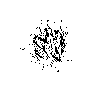
\includegraphics[width=52mm]{2005-gtq-ps3-2.eps}&
\includegraphics[width=52mm]{2005-gtq-ps3-4.eps}\\
\includegraphics[width=52mm]{2005-gtq-ps4-0.eps}&
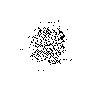
\includegraphics[width=52mm]{2005-gtq-ps4-2.eps}&
\includegraphics[width=52mm]{2005-gtq-ps4-4.eps}\\
\end{tabular}

\caption{Sets of angles $\hat \theta$ [rad] for joint measurements in one plane
where the probability for measuring a certain sum of outcomes is the same as for
unentangled particles; $\tau = 0$~($\vert \Psi_{4,s_1} \rangle$),
$\tau = \frac{\pi}{6}$,
$\tau = \frac{\pi}{3}$ and
$\tau = \frac{\pi}{2}$~($\vert \Psi_{4,s_2} \rangle$).}
\label{2005-gtq-plots2}
\end{figure}


Because of the spherical symmetry of the singlet state,
the probabilities for negative sums of outcomes are the same as
for positive sums. Furthermore, for measuring all particles along the same angle
($\theta_2 - \theta_1 = \theta_3 - \theta_1 = \theta_4 - \theta_1 = 0$ in
Fig.~\ref{2005-gtq-plots2}) applies $P_{sum=0}=1$ and $P_{sum=\pm4,\pm2}=0$.
As the sum of outcomes equals $\pm 2$ if and only if the four particles were found
in an odd number of spin-``$-$''-states,
\begin{equation}
P_{{\rm sum}=\pm 2}=\frac{1}{2} P_{{\rm odd}}=\frac{1}{4} \left( 1-E \right),
\label{2005-gtq-psum2}
\end{equation}
and the corresponding plots in Fig.~\ref{2005-gtq-plots1} and Fig.~\ref{2005-gtq-plots2}
are equivalent.

%We conclude by pointing out that the expectation functions of four-partite singlet states
%have a great variability.
We conclude by pointing out that all configurations discussed above could, for instance, be locally realized
by generalized beam splitters \cite{rzbb}.
Nonetheless, it would be interesting to test quantum mechanical predictions in a nonlocal setup.
As could have been expected,
without selection it is impossible to construct ``stronger--than''
(such as the one discussed in  Ref.~\cite{svozil-2004-brainteaser}) two-particle quantum correlations even for ``condensed'' four--partite correlations.
We conjecture that this remains true for an arbitrary number of quanta,
although ``stronger--than'' two-particle quantum correlations
are not forbidden by causality \cite{pop-rohr,popescu-97b,svozil-krenn}.




\begin{table}
\begin{tabular}{c}
\hline\hline
Two-partite singlet state\\
%\hline
$
E(\theta_1,\theta_2,\varphi_1 , \varphi_2)=P_= -P_{\neq }=
-\left[\cos \theta_1 \cos \theta_2 + \cos (\varphi_1 - \varphi_2) \sin \theta_1 \sin \theta_2\right]
$
\\
$
P_==
{1\over2}\left(1 + E  \right)
\; ,\;
P_{\neq} =
{1\over2}\left(1 - E \right)
$
\\
\hline
Four-partite singlet states\\
%\hline
$
P_{ \rm even} =
{1\over2}\left[1 + E  \right]
\; ,\;
P_{\rm odd} =
{1\over2}\left[1 - E  \right]
\; ,\;
E=
P_{{\rm even}}
-
P_{{\rm odd}}
$
\\
$E_{\rho_{ 1 }}({\hat \theta} )  =
\cos (\theta_1 -\theta_2 ) \cos (\theta_3 -\theta_4 ),
$
\\
$
\begin{array}{lll}
E_{\rho_{ 1 }}({\hat \theta} , {\hat \varphi } )  &=&
\left[\cos \theta_1 \cos \theta_2 +
          \cos ( \varphi_1 - \varphi_2) \sin \theta_1 \sin \theta_2\right]\cdot \\
&&\qquad  \qquad  \left[\cos \theta_3 \cos \theta_4 +
          \cos (\varphi_3 - \varphi_4) \sin \theta_3 \sin \theta_4
\right]
\end{array}
$
\\
$E_{\rho_{ 2 }}({\hat \theta} )  =
\frac{1}{3} \left[2 \cos (\theta_1 +\theta_2 -\theta_3 -\theta_4 )+\cos
   (\theta_1 -\theta_2 ) \cos (\theta_3 -\theta_4 )\right].
$
\\
$
\begin{array}{lll}
E_{\rho_{ 2 }}({\hat \theta} ,{\hat \varphi})  &=&
\frac{1}{3}
\left\{
\cos \theta_3 \sin \theta_1
\left[
-\cos \theta_4 \cos (\varphi_1 - \varphi_2) \sin \theta_2 +
          2 \cos \theta_2 \cos (\varphi_1 - \varphi_4) \sin \theta_4
\right] +
\right.
\\
&&\qquad
    \sin \theta_1 \sin \theta_3
\left[2 \cos \theta_2 \cos \theta_4 \cos (\varphi_1 - \varphi_3)  +
\right.
\\
&&\qquad
\qquad
\left.
\left(
2 \cos (\varphi_1 + \varphi_2 - \varphi_3 - \varphi_4) +
                \cos (\varphi_1 - \varphi_2)
                \cos (\varphi_3 - \varphi_4)
\right) \sin \theta_2 \sin \theta_4
\right]   +
\\
&&\qquad
    \cos \theta_1
\left[
2 \sin \theta_2
\left(
\cos \theta_4 \cos (\varphi_2 - \varphi_3) \sin \theta_3 +
                \cos \theta_3 \cos (\varphi_2 - \varphi_4) \sin \theta_4
\right) \right.
 +
\\
&&\qquad
\qquad
\left.
\left.
\cos \theta_2
\left(3 \cos \theta_3 \cos \theta_4 -
                \cos (\varphi_3 - \varphi_4) \sin \theta_3
\sin \theta_4
\right)
\right]
\right\}
\end{array}
$
\\
$
\begin{array}{lll}
E(\tau  ;{\hat \theta} )  &=&
\frac{1}{3}\left\{
\left[ 2 + \cos (2\,\tau  ) \right] \,\cos (\theta_1  - \theta_2 )\,\cos (\theta_3  - \theta_4 )+
 \right.  \\
&& \qquad \; \left. + 2\,\sin \tau
         \left[\sin \tau  \,\cos (\theta_1  + \theta_2  - \theta_3  - \theta_4 ) +
       {\sqrt{3}}\,\cos \tau  \,\sin (\theta_1  - \theta_2 )\,\sin (\theta_3  - \theta_4 ) \right]
\right\}
\end{array}
$
\\
$
\begin{array}{lll}
E(\tau  ;{\hat \theta},{\hat \varphi} )  &=&
\frac{1}{3} \left\{\cos \theta_1  \left(\cos \theta_2  \{3  \cos \theta_3  \cos \theta_4 +[2 \cos (2 \tau )+1]  \cos (\varphi_3-\varphi_4) \sin    \theta_3  \sin \theta_4 \}+ \right. \right. \\
&& \qquad  \qquad
2 \sin \theta_2  \sin \tau  \left[\cos \theta_3  \cos (\varphi_2-\varphi_4) \sin \theta_4 \left(\sqrt{3} \cos \tau +\sin \tau \right)- \right. \\
&& \qquad  \qquad
\left. \left.
\cos \theta_4  \cos (\varphi_2-\varphi_3) \sin \theta_3  \left(\sqrt{3} \cos \tau -\sin \tau \right)\right]\right)+\\
&& \qquad
\sin \theta_1 \left(\cos \theta_3  \left\{\cos \theta_4  [2 \cos (2 \tau )+1] \cos (\varphi_1-\varphi_2) \sin \theta_2 + \right.\right.\\
&&   \qquad  \qquad
\left.
2 \cos \theta_2  \cos (\varphi_1-\varphi_4) \sin \theta_4  \sin \tau  \left(\sin \tau -\sqrt{3} \cos \tau \right)\right\}+\\
&&   \qquad  \qquad
\sin \theta_3  \left[2 \cos \theta_2  \cos \theta_4  \cos (\varphi_1-\varphi_3) \sin \tau  \left(\sqrt{3} \cos \tau +\sin \tau \right)+\right.\\
&&   \qquad  \qquad
\sin \theta_2  \sin \theta_4  \left\{2 \cos (\varphi_1+\varphi_2-\varphi_3-\varphi_4) \sin ^2\tau +\right.\\
&&  \qquad  \qquad
\left.  \left. \left. \left.
[\cos (2 \tau )+2] \cos (\varphi_1-\varphi_2)\cos (\varphi_3-\varphi_4)+\sqrt{3} \sin (2 \tau ) \sin (\varphi_1-\varphi_2) \sin (\varphi_3-\varphi_4)
\right\}\right]\right)\right\}
\end{array}
$
\\
\hline\hline
\end{tabular}
\caption{Probabilities and expectation functions
for finding an odd or even number of spin-``$-$''-states.
\label{2005-gtq-2part}
}
\end{table}

\begin{table}
\begin{tabular}{c}
\hline\hline
Three-partite GHZM state (Ref.~\cite{krenn1})\\
$
P_\pm  =
{1\over 4}\left[1 + 2 E  \right]
\; ,\;
P_\pm  =
{1\over 4}\left[1 - 2 E  \right]
\; ,\;
E_\pm =
P_\pm
-
P_\pm
$
\\
$E_\pm (\theta_1,\theta_2,\theta_3,\varphi_1, \varphi_2,\varphi_3 \vert \pm_3)  =
\frac{1}{2}\left[
\cos \theta_1 \cos \theta_2
  \pm_3 \cos \left(\varphi_1 + \varphi_2 + \varphi_3\right)
\sin \theta_1 \sin \theta_2 \sin \theta_3
\right]$\\
%\hline
\hline
Four-partite singlet states\\
$
E_{\rho_{ 2 }}({\hat \theta} ,{\hat \varphi}\vert \pm_4)=   \frac{1}{12}
\pm {1\over 2} E_{\rho_{ 2 }}({\hat \theta} ,{\hat \varphi})
$   \\
$
E_{\rho_{ 2 }}({\hat \theta} \vert \pm_3 \pm_4)=   \frac{1}{12}\left\{2 (\pm_3 1) (\pm_4 1) \cos (\theta_1 + \theta_2 - \theta_3 - \theta_4) +
    \cos (\theta_1 - \theta_2) \left[1 + (\pm_3 1) (\pm_4 1) \cos (\theta_3 - \theta_4)\right]\right\}
$   \\
$
\begin{array}{lll}
E_{\rho_{ 2 }}({\hat \theta} ,{\hat \varphi}\vert \pm_3 \pm_4)&=&  \frac{1}{12}
\left\{\cos \theta_1 (2 (\pm_3 1) (\pm_4 1) \sin \theta_2 \left[\cos \theta_4 \cos (\varphi_2 - \varphi_3) \sin \theta_3 + \right. \right.
\\ && \qquad
\left.
                \cos \theta_3 \cos (\varphi_2 - \varphi_4) \sin \theta_4\right] +
\\ && \qquad
                \cos \theta_2 \left[1 + 3 (\pm_3 1) (\pm_4 1) \cos \theta_3 \cos \theta_4 -         \right.
\\ && \qquad
\left.
                (\pm_3 1) (\pm_4 1) \cos (\varphi_3 - \varphi_4) \sin \theta_3 \sin \theta_4\right]) +
\\ && \qquad
                \sin \theta_1 (\cos (\varphi_1 - \varphi_2) \sin \theta_2 \left[1 - (\pm_3 1) (\pm_4 1) \cos \theta_3 \cos \theta_4 +\right.
\\ && \qquad
\left.
                (\pm_3 1) (\pm_4 1) \cos (\varphi_3 - \varphi_4) \sin \theta_3 \sin \theta_4\right] +
\\ && \qquad
                2 (\pm_3 1) (\pm_4 1) \left[\cos \theta_2 \cos \theta_4 \cos (\varphi_1 - \varphi_3) \sin \theta_3 +\right.
\\ && \qquad
                \cos \theta_2 \cos \theta_3 \cos (\varphi_1 - \varphi_4) \sin \theta_4 +
\\ && \qquad
\left.
\left.
\left.
                \cos (\varphi_1 + \varphi_2 - \varphi_3 - \varphi_4) \sin \theta_2 \sin \theta_3 \sin \theta_4\right]\right)\right\}
\end{array}$   \\
$
E_{\rho_{ 2 }}({\hat \theta} \vert \pm_2 \pm_4)=   \frac{1}{12}\left\{
     (\pm_2 1) (\pm_4 1) \left[2 \cos (\theta_1 + \theta_2 - \theta_3 - \theta_4) +
          \cos (\theta_1 - \theta_2) \cos (\theta_3 - \theta_4)\right]
-2 \cos (\theta_1 - \theta_3)
\right\}
$   \\
$
\begin{array}{lll}
E_{\rho_{ 2 }}({\hat \theta} ,{\hat \varphi}\vert \pm_2 \pm_4)&=&  \frac{1}{12}
\left\{\cos \theta_1 ((\pm_2 1) (\pm_4 1) \sin \theta_3 \left[2 \cos \theta_4 \cos (\varphi_2 - \varphi_3) \sin \theta_2 -  \right.\right.
\\ && \qquad
\left.
                \cos \theta_2 \cos (\varphi_3 - \varphi_4) \sin \theta_4\right] +
\\ && \qquad
           \cos \theta_3 \left[-2 + 3 (\pm_2 1) (\pm_4 1) \cos \theta_2 \cos \theta_4 + \right.
\\ && \qquad
\left.
                2 (\pm_2 1) (\pm_4 1) \cos (\varphi_2 - \varphi_4) \sin \theta_2 \sin \theta_4\right]) +
\\ && \qquad
    \sin \theta_1 ((\pm_2 1) (\pm_4 1) \cos \theta_3 \left[-\cos \theta_4 \cos (\varphi_1 - \varphi_2) \sin \theta_2 +\right.
\\ && \qquad
\left.
                2 \cos \theta_2 \cos (\varphi_1 - \varphi_4) \sin \theta_4\right] +
\\ && \qquad
          \sin \theta_3 (2 \left[-1 + (\pm_2 1) (\pm_4 1) \cos \theta_2 \cos \theta_4\right] \cos (\varphi_1 - \varphi_3) +
\\ && \qquad
                (\pm_2 1) (\pm_4 1) (2 \cos (\varphi_1 + \varphi_2 - \varphi_3 - \varphi_4) +
\\ && \qquad
\left.
                      \cos (\varphi_1 - \varphi_2) \cos (\varphi_3 - \varphi_4)) \sin \theta_2 \sin \theta_4))\right\}
\end{array}$   \\
\hline\hline
\end{tabular}
\caption{Probabilities and expectation functions
for finding an odd or even number of spin-``$-$''-states,
with selection.
\label{2005-gtq-2partwith}
}
\end{table}

\begin{table}

\begin{equation*}
\begin{split}
P^{{\rm sum}=0}_{\rho_1} ({\hat \theta} ,{\hat \varphi}) =& \frac{1}{48}
\Bigl[ 6 \cos \left( \varphi_1 - \varphi_2\right)
\left( 1 + 3 \cos \theta_3 \cos \theta_4 \right) \sin \theta_1 \sin \theta_2 +
4 \cos \left(\varphi_3 - \varphi_4\right) \sin \theta_3 \sin \theta_4\\
&+ 12 \cos \left(\varphi_3 - \varphi_4\right) \cos \theta_1
\cos \theta_2 \sin \theta_3 \sin \theta_4 + 2 \cos \left(\varphi_3 - \varphi_4\right)
\left( 1 + 3 \cos \theta_1 \cos \theta_2 \right) \sin \theta_3 \sin \theta_4\\
&+ 6 \bigl( 3 + \cos \theta_3 \cos \theta_4 + \cos \theta_1 \cos \theta_2
\left( 1 + 3 \cos \theta_3 \cos \theta_4 \right)\\
&+ 3 \cos \left(\varphi_1 - \varphi_2\right) \cos \left(\varphi_3 - \varphi_4\right)
\sin \theta_1 \sin \theta_2 \sin \theta_3
\sin \theta_4 \bigr) \Bigr]
\end{split}
\end{equation*}
\begin{equation*}
\begin{split}
P^{{\rm sum}=2}_{\rho_1} ({\hat \theta} ,{\hat \varphi}) =& P^{{\rm sum}=-2}_{\rho_1}
({\hat \theta} ,{\hat \varphi}) = \frac{1}{24}
\Bigl[ -6 \cos \left( \varphi_1 - \varphi_2\right) \cos \theta_3 \cos \theta_4 \sin \theta_1 \sin \theta_2\\
&- 6 \cos \left(\varphi_3 - \varphi_4 \right) \cos \theta_1 \cos \theta_2 \sin \theta_3 \sin \theta_4
- 6 \bigl( \cos \theta_1 \cos \theta_2 \cos \theta_3 \cos \theta_4\\
&+ \cos \left(\varphi_1 - \varphi_2\right) \cos \left(\varphi_3 - \varphi_4\right)
\sin \theta_1 \sin \theta_2 \sin \theta_3 \sin \theta_4 - 1 \bigr) \Bigr]
\end{split}
\end{equation*}
\begin{equation*}
\begin{split}
P^{{\rm sum}=4}_{\rho_1} ({\hat \theta} ,{\hat \varphi}) =& P^{{\rm sum}=-4}_{\rho_1}
({\hat \theta} ,{\hat \varphi}) = \frac{1}{96}
\Bigl[ 6 \cos \left( \varphi_1 - \varphi_2\right) \bigl( \cos \theta_3 \cos \theta_4 - 1 \bigr)
\sin \theta_1 \sin \theta_2\\
&- 4 \cos \left( \varphi_3 - \varphi_4 \right) \sin \theta_3 \sin \theta_4 + 4
\cos \left( \varphi_3 - \varphi_4 \right) \cos \theta_1 \cos \theta_2 \sin \theta_3 \sin \theta_4\\
&+ 2 \cos \left( \varphi_3 - \varphi_4 \right) \bigl( \cos \theta_1 \cos \theta_2 -1 \bigr)
\sin \theta_3 \sin \theta_4 + 6 \Bigl( \bigl( \cos \theta_1 \cos \theta_2 - 1 \bigr)\\
&\cdot \bigl( \cos \theta_3 \cos \theta_4 - 1 \bigr) + \cos \left( \varphi_1 - \varphi_2 \right)
\cos \left( \varphi_3 - \varphi_4 \right) \sin \theta_1 \sin \theta_2 \sin \theta_3 \sin \theta_4 \Bigr) \Bigr]
\end{split}
\end{equation*}

\caption{Probabilities for all possible sums of outcomes of spin state measurements
(``$+$'' and ``$-$'' counted as $+1$ and $-1$, respectively) on 4 particles in the
singlet state $\vert \Psi_{4,s_1} \rangle$
%($\tau = 0$)
.}
\label{2005-gtq-tabsums1}

\end{table}


\begin{table}

\begin{equation*}
\begin{split}
P^{{\rm sum}=0}_{\rho_2} ({\hat \theta} ,{\hat \varphi}) =& \frac{1}{48}
\Bigl[ - 4 \cos \left( \varphi_3 - \varphi_4 \right) \sin \theta_3 \sin \theta_4
- 12 \cos \left( \varphi_3 - \varphi_4 \right) \cos \theta_1 \cos \theta_2 \sin \theta_3 \sin \theta_4
+ 2 \cos \left( \varphi_3 - \varphi_4 \right)\\
&\cdot \left( 3 \cos \theta_1 \cos \theta_2 + 1 \right) \sin \theta_3 \sin \theta_4
+ 2 \cos \left( \varphi_1 - \varphi_2 \right) \sin \theta_1 \sin \theta_2
\Bigl( 3 \cos \left( \varphi_3 - \varphi_4 \right) \sin \theta_3 \sin \theta_4\\
&- 3 \cos \theta_3 \cos \theta_4 - 1 \Bigr)
+ 2 \Bigl( 2 \cos \theta_2 \cos \theta_3 - \cos \theta_3 \cos \theta_4 + 2 \cos \theta_2 \cos \theta_4
+ 2 \cos \left( \varphi_1 - \varphi_3 \right)\\
&\cdot \sin \theta_1 \sin \theta_3 + 6 \cos \left( \varphi_1 - \varphi_3 \right)
\cos \theta_2 \cos \theta_4 \sin \theta_1 \sin \theta_3
+ 2 \cos \left( \varphi_2 - \varphi_3 \right) \sin \theta_2 \sin \theta_3\\
&+ 2 \bigl\{ \cos \left( \varphi_1 - \varphi_4 \right) \left( 3 \cos \theta_2 \cos \theta_3 + 1 \right)
\sin \theta_1 + \sin \theta_2 \bigl[ \cos \left( \varphi_2 - \varphi_4 \right)
+ 3 \cos \left( \varphi_1 + \varphi_2 - \varphi_3 - \varphi_4 \right)\\
&\cdot \sin \theta_1 \sin \theta_3 \bigr] \bigr\} \sin \theta_4
+ \cos \theta_1 \bigl\{ 2 \left( \cos \theta_3 + \cos \theta_4 \right)
+ \cos \theta_2 \left( 9 \cos \theta_3 \cos \theta_4 - 1 \right)
+ 6 \sin \theta_2\\
&\cdot \bigl[ \cos \left( \varphi_2 - \varphi_3 \right) \cos \theta_4 \sin \theta_3
+ \cos \left( \varphi_2 - \varphi_4 \right) \cos \theta_3 \sin \theta_4 \bigr]
\bigr\} \Bigr) + 18 \Bigr]
\end{split}
\end{equation*}
\begin{equation*}
\begin{split}
P^{{\rm sum}=2}_{\rho_2} ({\hat \theta} ,{\hat \varphi}) =& P^{{\rm sum}=-2}_{\rho_2}
({\hat \theta} ,{\hat \varphi}) = \frac{1}{24}
\Bigl[ 2 \cos \left( \varphi_3 - \varphi_4 \right)
\cos \theta_1 \cos \theta_2 \sin \theta_3 \sin \theta_4
- 2 \cos \left( \varphi_1 - \varphi_2 \right) \sin \theta_1 \sin \theta_2\\
&\cdot \Bigl( \cos \left( \varphi_3 - \varphi_4 \right) \sin \theta_3 \sin \theta_4
- \cos \theta_3 \cos \theta_4 \Bigr) - 2 \Bigl( \cos \theta_4 \bigl\{
3 \cos \theta_1 \cos \theta_2 \cos \theta_3 + 2 \bigl[ \cos \left( \varphi_1 - \varphi_3 \right)\\
&\cdot \cos \theta_2 \sin \theta_1 \cos \left( \varphi_2 - \varphi_3 \right)
\cos \theta_1 \sin \theta_2 \bigr] \sin \theta_3 \bigr\}
+ 2 \bigl\{ \cos \left( \varphi_1 - \varphi_4 \right) \cos \theta_2 \cos \theta_3 \sin \theta_1\\
&+ \cos \left( \varphi_1 + \varphi_2 - \varphi_3 + \varphi_4 \right)
\sin \theta_1 \sin \theta_2 \sin \theta_3 \cos \left( \varphi_2 - \varphi_4 \right)
\cos \theta_1 \cos \theta_3 \sin \theta_2 \bigr\} \sin \theta_4 - 3 \Bigr) \Bigr]
\end{split}
\end{equation*}
\begin{equation*}
\begin{split}
P^{{\rm sum}=4}_{\rho_2} ({\hat \theta} ,{\hat \varphi}) =& P^{{\rm sum}=-4}_{\rho_2}
({\hat \theta} ,{\hat \varphi}) = \frac{1}{96}
\Bigl[ 4 \cos \left( \varphi_3 - \varphi_4 \right) \sin \theta_3 \sin \theta_4
-4 \cos \left( \varphi_3 - \varphi_4 \right) \cos \theta_1 \cos \theta_2 \sin \theta_3 \sin \theta_4\\
&+ 2 \cos \left( \varphi_3 - \varphi_4 \right) \left( \cos \theta_1 \cos \theta_2 - 1 \right)
\sin \theta_3 \sin \theta_4 + 2 \cos \left( \varphi_1 - \varphi_2 \right) \sin \theta_1 \sin \theta_2
\Bigl( \cos \left( \varphi_3 - \varphi_4 \right)\\
&\cdot \sin \theta_3 \sin \theta_4
- \cos \theta_3 \cos \theta_4 + 1 \Bigr) + 2 \Bigl(
\cos \theta_3 \cos \theta_4 - 2 \cos \theta_2 \cos \theta_3 - 2 \cos \theta_2 \cos \theta_4\\
&- 2 \cos \left( \varphi_1 - \varphi_3 \right) \sin \theta_1 \sin \theta_3
+ 2 \cos \left( \varphi_1 - \varphi_3 \right) \cos \theta_2 \cos \theta_4 \sin \theta_1 \sin \theta_3
- 2 \cos \left( \varphi_2 - \varphi_3 \right)\\
&\cdot \sin \theta_2 \sin \theta_3 + 2 \bigl\{ \sin \theta_1
\bigl[ \cos \left( \varphi_1 - \varphi_4 \right) \left( \cos \theta_2 \cos \theta_3 - 1 \right)
+ \cos \left( \varphi_1 + \varphi_2 - \varphi_3 + \varphi_4 \right) \sin \theta_2 \sin \theta_3 \bigr]\\
&- \cos \left( \varphi_2 - \varphi_4 \right) \sin \theta_2 \bigr\} \sin \theta_4
+ \cos \theta_1 \bigl\{ 3 \cos \theta_2 \cos \theta_3 \cos \theta_4 + \cos \theta_2
- 2 \left( \cos \theta_3 + \cos \theta_4 \right)\\
&+ 2 \cos \left( \varphi_2 - \varphi_3 \right)
\cos \theta_4 \sin \theta_2 \sin \theta_3 + 2 \cos \left( \varphi_2 - \varphi_4 \right)
\cos \theta_3 \sin \theta_2 \sin \theta_4 \bigr\} \Bigr) + 6 \Bigr]
\end{split}
\end{equation*}


\caption{Probabilities for all possible sums of outcomes of spin state measurements
(``$+$'' and ``$-$'' counted as $+1$ and $-1$, respectively) on 4 particles in the
singlet state $\vert \Psi_{4,s_2} \rangle$
%($\tau = \pi / 2$)
.}
\label{2005-gtq-tabsums2}
\end{table}



{\bf Acknowledgments:}
Karl Svozil gratefully acknowledges discussions with G\"unther Krenn and Johann Summhammer in Viennese coffee houses and elsewhere.
%Many ideas emerged in those conversations and also during lonesome walks through the Vienna Woods.


\bibliography{svozil}
%\bibliographystyle{apsrev}
%\bibliographystyle{unsrt}
%\bibliographystyle{plain}
\bibliographystyle{osa}


\end{document}

